%
% Refrence http://en.wikibooks.org/wiki/LaTeX
%

\documentclass[10pt]{article}

% ======
% Header
% ======

% use droid sans
\usepackage{droidsans}    
\renewcommand\familydefault{\sfdefault}   % set default font to sans-serif


% enable \href
\usepackage[colorlinks=true,
            linkcolor=blue,
            urlcolor=blue,
            allbordercolors={0 0 0},
            pdfborderstyle={/S/U/W 1}]{hyperref}

% enable \includegraphics for embedding jpgs
\usepackage{graphicx}  

% ==================
% Document Meta Data
% ==================

\title{Webtech Report}
\author{Imna Malik n James Sewart}
\date{29-5-16}

% ====
% Body
% ====

\begin{document}

    \maketitle

    \tableofcontents


    \begin{abstract}
        visual music discovery service using data crawled from various apis and combined
    \end{abstract}

    \section{Client}
        \subsection{Style}
            \subsubsection{Base Classes}
                The design of our layout is inspired by Material Design, using card style boxes. Each panel is given a shadowbox class which gives the element a border radius, shadow, slight transparency, and a dark background colour. The search panel and all panels in the info bar are given this class.

            \subsubsection{Resizing}
                We use CSS media queries to resize the info panel stuff like the and basically and the seearch panel thats everything. The font resize thingy we use percentages and ems we basically use the media query thing we change the font size and have everything inside percentages so everythings dynamic

                We use CSS media queries to change large scale layouts based on the screen size. There are three of these: mobile-sized, large, and extra large. These changes involve setting the widths of the main panels such that they look good on the screen size. For the mobile screen this means the panels are full width and stack on top of each other. For the large size the info bar takes up a third of the screen, and the search 40\% of the screen.

                For a more dynamic resize control we subscribe to the onresize event of the window and scale the whole documents font size based on the screen width. Most elements are defined using ems and so they all scale accordingly.

            \subsubsection{General Layout}
                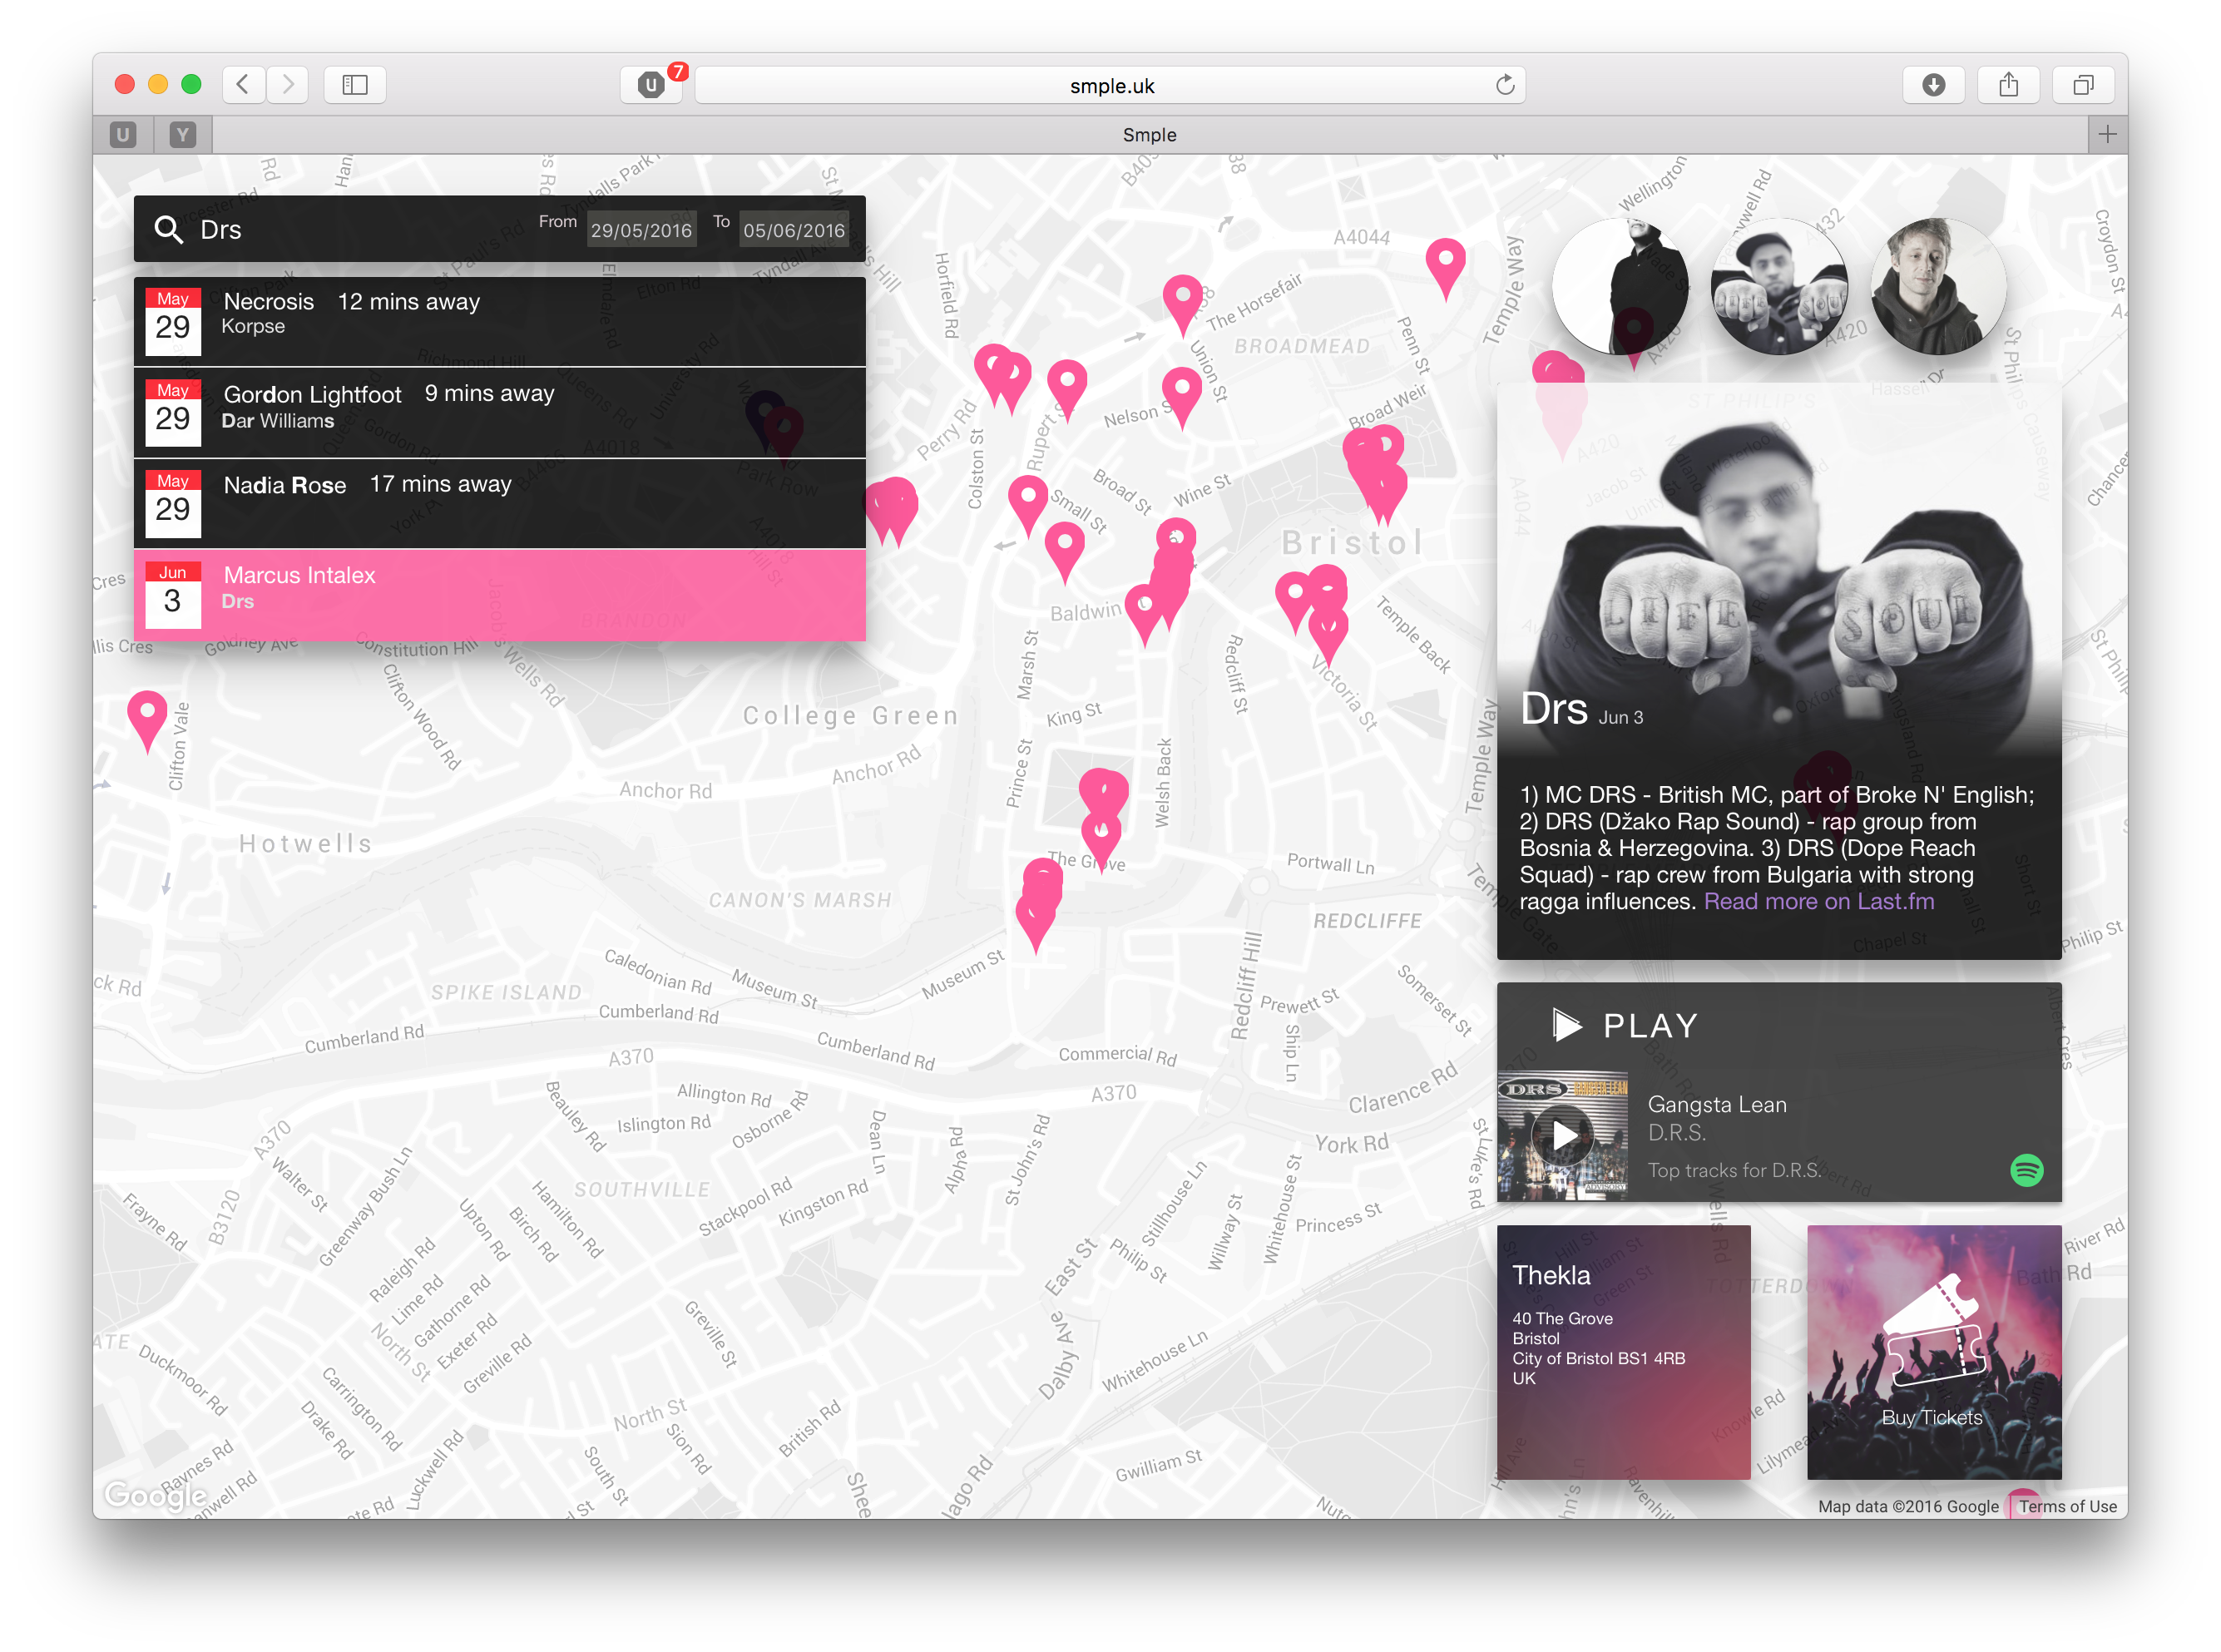
\includegraphics[height=60mm]{example1.png}
                \begin{itemize}
                    \item whole screen map, fixed
                    \item hud like overlay for interactions

                    \item fixed search panel on left third?
                    \item search results expand panel downwards dynamically

                    \item info panel on right third
                    \item info panel slides in on marker click
                    \item slides out on map move or zoom
                    \item panel scrolls on overflow, but not the whole page
                \end{itemize}

            \subsubsection{Info Panel}
                \begin{itemize}
                    \item css animations
                    \item place offscreen and disallow scrolling
                    \item fixed size to screen

                    \item top layer is a dynamic number of thumbnails for each band in an event
                        \begin{itemize}
                            \item animated and bevelled
                        \end{itemize}
                    \item second layer is the current band information
                        \begin{itemize}
                            \item text over image with transparency fade
                            \item paragraph after both
                            \item width is fixed, text on image is pinned to bottom of image, paragraph comes after image
                        \end{itemize}
                    \item third layer is a sample music button
                        \begin{itemize}
                            \item includes clickable svg and spotify player that is hidden intially
                            \item clicking the svg triggers an SMIL animation on parts of the svg, reveals the spotify player, and fades the background colour to match the player xO
                            \item clicking play again reverses these animations
                        \end{itemize}

                    \item fourth layer includes event information
                        \begin{itemize}
                            \item first box is location information with link to the songkick page for the venue
                            \item second box includes self made svg of tickets and is clickable to get to the ticket purchasing page
                            \item background image has been modified using gimp and is animated to fade on mouse over
                            \item took a long time to get these boxes in the desired position wewew
                        \end{itemize}
                \end{itemize}

            \subsubsection{Search Panel}
                \begin{itemize}
                    \item persistent search box with icon from a custom font
                    \item the google maps distance matrix api is used on the client side to determine how far away events are from the users current location, this is displayed with the search
                    \item a custom date icon was created using html and adds a nice visual to when event takes place, this is generated by javascript with the date and month injected in to be added to each search result
                    \item clicking on a search result repositions the map to see where it is and opens the relevant info panel
                \end{itemize}

            \subsubsection{Date Filter}
                \begin{itemize}
                    \item fixed up real nice calendar lib and made pull request n all \textless3
                    \item looks super dank in the search panel iluvit
                \end{itemize}

            \subsubsection{Map}
                \begin{itemize}
                    \item using the google maps api with a custom theme
                    \item adding markers for each event in our data structure
                    \item marker onclick opens the info bar for the desired event and centers the event, also animated the marker icon using googles animations
                    \item the marker icons are a custom svg designed by imna herself
                \end{itemize}


        \subsection{Logic}
            \begin{itemize}
                \item Initially the info panel is hidden and the map loads with an empty search panel overlayed
                \item the main script initiates a websocket connection with the server, and once both the map and the websocket connection is made, the client sends its current map position to the server.
                \item This triggers the server to send nearby events, which once received are visualised on the map as our custom markers.
                \item a user can then click a marker which triggers the sidepanel to be animated in and its content updated to match the information in the data structure for that event
                \begin{itemize}
                    \item this involved creating a dynamic number of band thumbnails and inserting it into the correct position
                    \item updating the band info box to the first band name and description, as well as updating the spotify player with the bands spotify link
                \end{itemize}
                \item the event name and location is updated as well as the links to the event page and the ticket buying page

                \item keyup in the search bar triggers search algorithm on nearby events which generates the results html
                \item results html is inserted inside a container div that is already there
                \item the search algorithm performs a sublime like fuzzy search by not matching sequential matches but each character can match any length into the text
                \item each matched character is given the bold html tag to signify that is the character that matched
            \end{itemize}

    \section{Server}
        The server uses the provided script with modifications. The index is served as a static file and dynamic content is achieved using Websocket connections between the client and server. This design choice simplifies the file resource serving logic, reducing the dynamic parts to message passing.

        Once the client has initialised the webpage, it sets up a secure Websocket connection to the server. A secure socket is preferred as non secure sockets are disallowed when viewing the page over https. The connection is abstracted into websocket.js such that server.js can simply pass a callback that is called when a new client query is made, with a parameter that can be called with the result to send back. server.js doesnt need to worry about managing connections.

        The client will query the browser for its current geographical location and when given, will send this to the server along with a desired date range. The server will reply at some point in the future with an array of events.

        The server will receive this data and use it to query the database using a geoNear query on a \href{https://docs.mongodb.com/manual/core/2dsphere/}{2dsphere} index, and a date range query on the event date. The results are sent to the client.

        Websockets provide a stream of messages, where a message is either some binary data or a string. We serialize JSON for sending data between the client and server. When the client sends its position and desired date range we serialize a data structure that looks like the following.

        \begin{verbatim}
        {
            pos: {
                lat: Number,
                lng: Number
            },
            dateRange: {
                from: Date,
                to: Date
            }
        }
        \end{verbatim}

        Dates aren't parsed into JavaScript date objects when using a JSON.parse so these are handled manually for the database queries.

        As well as giving the client the desired data we have, we also check whether the database needs updating. The data is collected using a variety of APIs. First we ask songkick for the area that the user is in, this allows us to check the database to see if we have checked this area at all/recently. If we haven't got an up to date set of events for this area, we start downloading the events for the area as well as querying last.fm for the artists biography and picture, spotify for a reference to their spotify page, and googles reverse geocode api to get the full address of the venue.

        For each area we limit the speed of requests in order to avoid rate limiting. Any returned errors by the APIs are handled graciously. Once complete data about an event is retrieved, it is stored in the database using an \href{https://docs.mongodb.com/manual/reference/method/db.collection.update/#upsert-option}{upsert} on the event title, to either update an already queried event, or insert as a new event.

        A possible optimization of the client-server interaction process would be to determine what events have already been sent to the client in order to avoid sending them again if they only scroll the map slightly. This would allow for significantly less data to be transferred between the two and would avoid reprocessing every event on the client side on every query change.


    \section{Deployment}
        \begin{itemize}
            \item by default server connects to a local mongodb instance and runs on the latest nodejs.
            \item This favours a vps installations on services like digitalocean or aws by simply cloning the git repo, performing an npm install and running both mongodb and the server script.
            \item the site is live at https://smple.uk
            \item git
        \end{itemize}

    \section{API}
        \begin{itemize}
            \item We made efforts to abide by the api tos by rate limiting and providing * where requested
            \item songkick-spotify-google-last.fm
        \end{itemize}


    % \begin{verbatim}
    %     j = []
    %     for i in range(10):
    %       j.append(i)
    %       j.append(i+1)
    %       j.append(i+2)
    %     sum(j)
    % \end{verbatim}


    % \subsection{Raw pictures}
    % \includegraphics[height=60mm]{moon.jpg}

    % \subsection{Figures}
    % \begin{figure}[!ht]
    %   \centering
    %     \reflectbox{%
    %       \includegraphics[width=0.5\textwidth]{moon.jpg}}
    %   \caption{A picture of the same gull
    %            looking the other way!}
    % \end{figure}

    % \section{Hyperlinks}
    % \href{http://www.google.com}{Ut enim}

    % \section{Tables}

    % \begin{tabular}{ l | c | r }
    %   \hline
    %   1 & 2 & 3 \\ \hline
    %   4 & 5 & 6 \\ \hline
    %   7 & 8 & 9 \\ \hline
    % \end{tabular}


    %
    % Footnotes
    % 
    % \section{Footnotes}
    % This is an example footnote\footnote{An example footnote.}
    % \footnotetext[17]{This is my footnote!}

    % \footnotemark[17]




\end{document}


